\chapter{Analysis and Conclusions}
\label{analysis}

% answer subquestion one: what patterns can be found using wavelet analysis?
\section{Sequence analysis}
There are more than 100,000 times more similar sequences found in the
scale/filter coefficients than in the wavelet/shift coefficients. The large
difference in number of sequences found between the two types of coefficients
is due to the fact that the LOC metric is a cumulative metric. The typical shape
of the LOC metric is a growing line. This makes finding a matching sequence of
coefficients using only shift coefficients (i.e., along the time axis) less
likely.

\paragraph{}
The fact that, of the 16,049 patterns, there are 0 patterns found in shift
coefficients was to be expected. The 16 similar sequences in shift coefficients
are not similar within the same group of sequences. Additionally, the shift
coefficients are incomparable to the filter coefficients because it is a
fundamentally different way of signal transformation. Mixing both types of
coefficients would ignore how the coefficients were found and invalidate the
patterns.

\section{Pattern evaluation}
\label{section:pattern_evaluation}
To be able to know what the patterns represent, the 16,049 patterns are
projected onto the original signal. This is done by finding the project the
pattern was first detected, and taking the pattern's level of decomposition and
starting point in the series of coefficients for its project.

As the set of values of level of decomposition, starting point in the series,
its length (i.e., number of coefficients), and the originating project is
unique for each pattern, it can be 're-projected' onto the signal of that
particular project. This gives the $age\_in\_months$ values the sequence starts
and ends in the project.

Knowing the start and end month of a sequence within a project, the values of
the original signal during the sequence are captured for further analysis.

\paragraph{}
The absolute maximum differences of the LOC values is computed for each
sequence. The patterns have maximum LOC differences between 0 (i.e., no change
in LOC in the sequence) and 6,862,111. Figure \ref{figure:pattern_loc_diff}
shows the distribution of this number across the patterns.

\begin{figure}[H]
\caption{Distribution of maximum LOC differences across
patterns}\label{figure:pattern_loc_diff}
\centering
	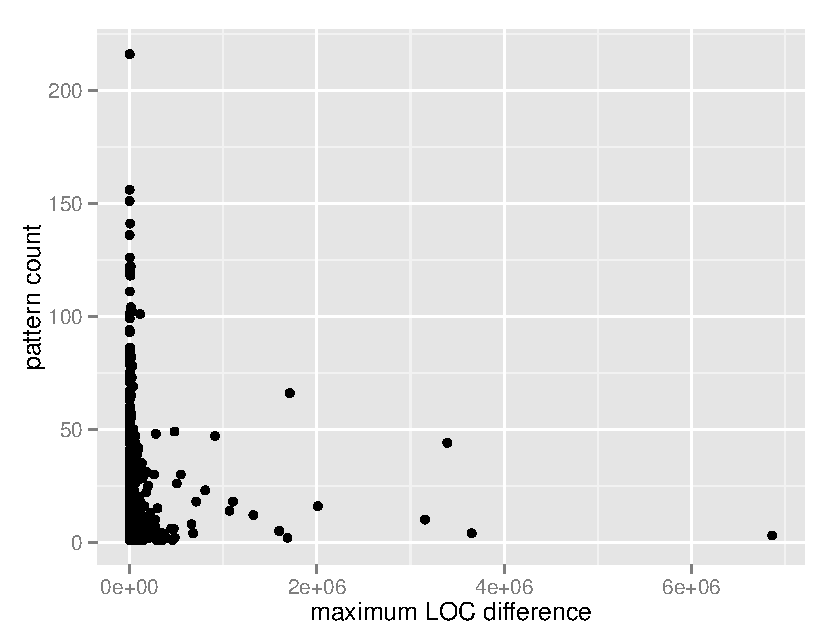
\includegraphics[width=296pt]{images/pattern_LOC_diff_100.pdf}
\end{figure}

75\% of the patterns have a maximum LOC difference less than 20,595; 50\% have
a maximum LOC difference less than 5,250; and 25\% less than 1,046.

\paragraph{}
The top four patterns with least maximum LOC differences are shown in Figure
\ref{figure:top_patterns_plots} to illustrate how such patterns look like. The
figure depicts the wavelets of the patterns for all the project signals they
were detected in. Which are the differences in LOC values between two subsequent
coefficients.

The graphs show that the sequences have similar waveforms. Each graph contains
a multiple of plotted sequences: pattern 1: 216 sequences; pattern 2: 156
sequences; pattern 3: 151 sequences; and pattern 4: 141 sequences. Note that
the factor of scale is reintroduced, because the sequences all contain
scale/filter coefficients. The factor of time, however, is still being
eliminated, hence the use of \emph{index }\rm instead of a time metric on the
horizontal axis.

\begin{figure}[H]
\caption{The four most common type A patterns projected onto original
signal}\label{figure:top_patterns_plots}
\centering
	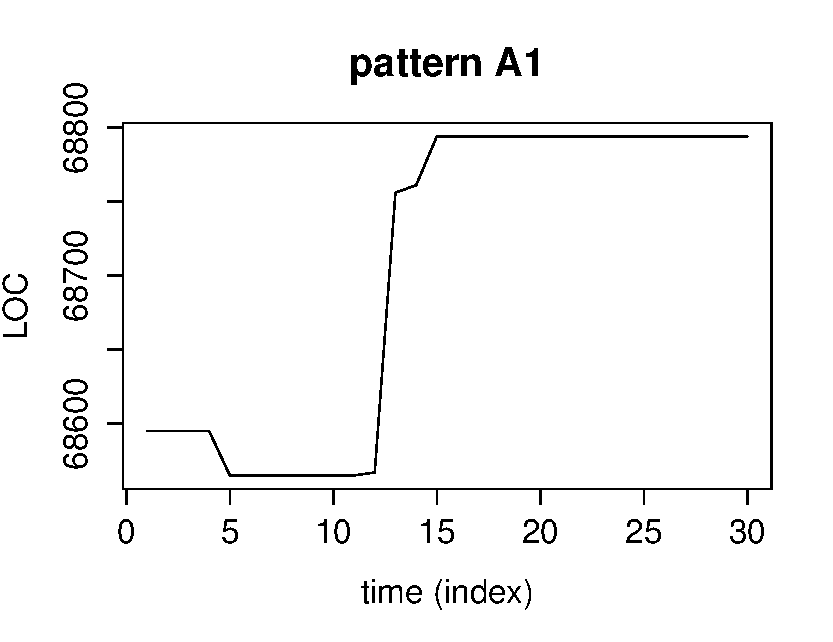
\includegraphics[width=196pt]{images/pattern_a1.pdf}
	\hspace{1em}
	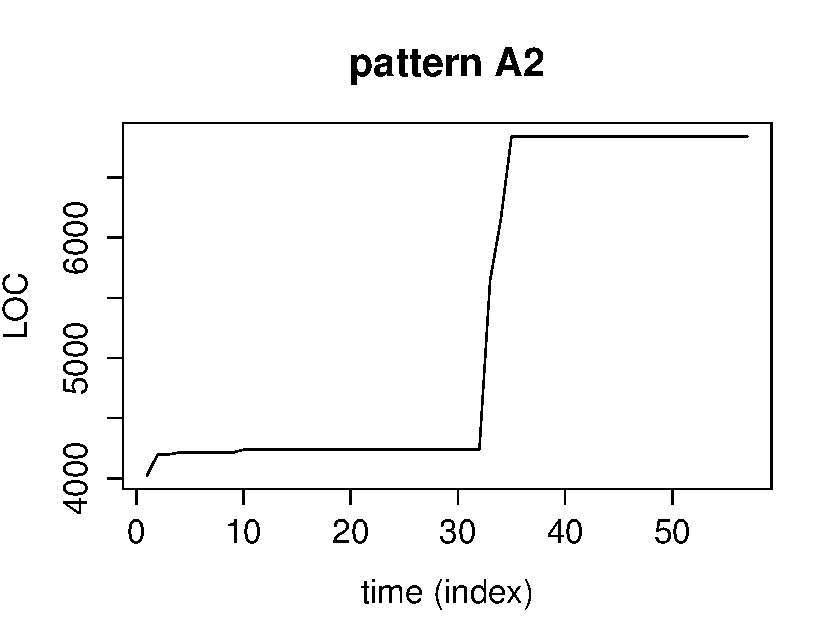
\includegraphics[width=196pt]{images/pattern_a2.pdf}
	\\
	\vspace{1em}
	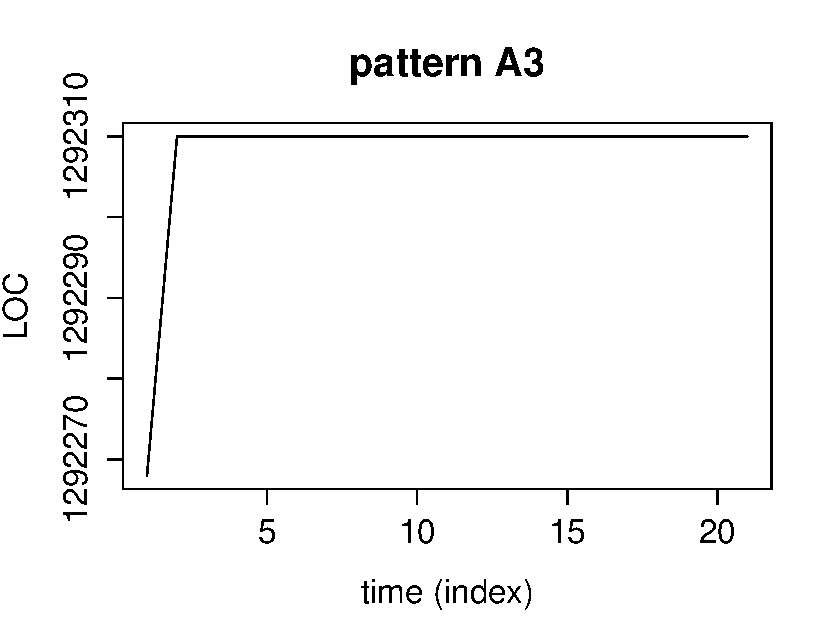
\includegraphics[width=196pt]{images/pattern_a3.pdf}
	\hspace{1em}
	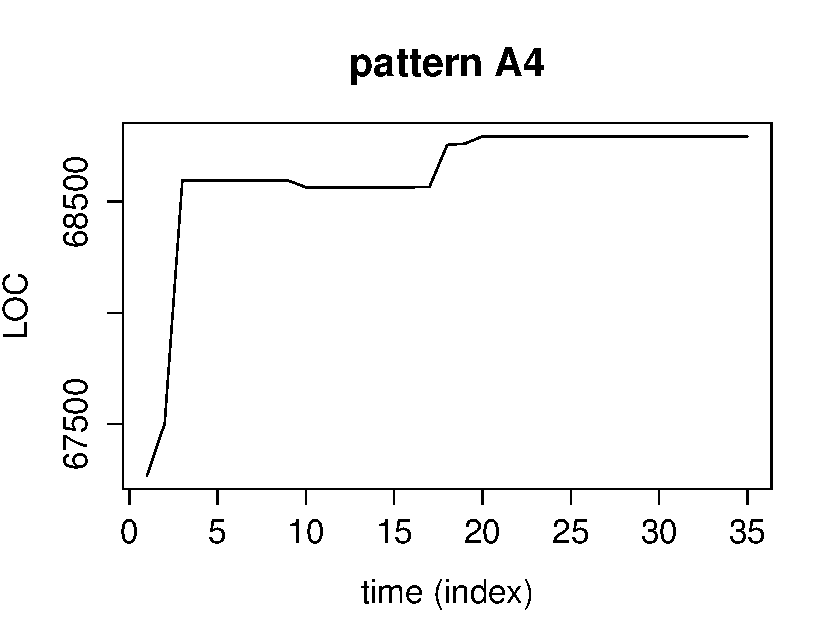
\includegraphics[width=196pt]{images/pattern_a4.pdf}
\end{figure}

\section{Conclusions}
%Many more sequences were found using filtering. This is expected as scaling is
% better than shifting at finding small coefficients.

\section{Threats to validity}
\begin{comment}
* Is the Ohloh database a representation of the world of OSS projects?
* Is LOC as the sum of source lines of code, comments, and blank lines valid?
* The use of LOC as a measure of project evolution. Does it represent
activity/growth/whatever to say something about the project's status?
* A selection criterion for the projects was a continuous series of subsequent
monthly facts. Maybe the full series of evolution data of a project is needed in
order to find objective signs or to be able to compare different projects.
* Is 250 projects enough to detect patterns and generalise to the world of OSS
projects?
* Is monthly aggregated data fine-grained enough?

\end{comment}

\section{Future work}


\begin{comment}
- Analyse results
- Conclude and interpret results
- Answer research questions
- Threats to validity
- Discussion
- Future work
 
This chapter contains the analysis and interpretation of the results. The
research questions are answered as best as possible given the results that were
obtained. The analysis also discussed parts of the questions that were left
unanswered.

An important topic is the validity of the results.
What methods of validation were used?
Could the results be generalized to other cases?
What threats to validity can be identified?

There is room here to discuss the results of related scientific literature here
as well.
How do the results obtained here relate to other work, and what consequences are
there?
Did your approach work better or worse?
Did you learn anything new compared to the already existing body of knowledge?
Finally, what could you say in hindsight on the research approach by followed?
What could have done better?
What lessons have been learned?
What could other researchers use from your experience?

A separate section should be devoted to ‘future work,’ i.e., possible extension
points of your work that you have identified. Other researchers (or yourself)
could use those as a starting point.

Refer to Chapters 3.7 and 4 in this example thesis at Paul’s
homepage\footnote{http://homepages.cwi.nl/~paulk/thesesMasterSoftwareEngineering/2006/ReneWiegers.pdf}.
\end{comment}
